% demo template available at the rapptorlab (Laurent Segers)
% this demo makes use of the VUB styling provided by Ruben De Smet
% Link for the VUB frontpage: https://gitlab.com/rubdos/texlive-vub 

%\documentclass[english]{book_template}
\documentclass[english]{book_template} % use this to have the book template as used by Laurent Segers
% start making up the title page
\title{Benchmarking single board computers for embedded systems}
%\subtitle{Course/thesis example} 
\author {Zineddine Wakrim} % Who am I?
\faculty{Engineering science} % place here faculty name (without placing the word Faculty)
\promotors{Jan Lemeire} % comment out if not thesis
\pretitle{In order to be awarded the Master's Degree in industrial science: Electronic-ICT with specialization embedded systems}

\def\triangleH{27.7mm}
% end of title page setup

\addbibresource{IEEEexample.bib}
\begin{document}
% do not remove the line below, makes the frontpage
\maketitle
% end of title page  
\newpage
  \null
\chapter*{Abstract}
\newpage
  \null
\chapter*{Acknowledgements}

\newpage
  \null

\tableofcontents
\listoffigures
\listoftables

\newpage
  \null

\chapter{Introduction} % use \chapter*{Inleiding} with asterix to have the title without number

This thesis will benchmark vision algorithms on several single board computers. The purpose of the thesis is to check how good a single board computer can do some real time image processing. 

Vision is a hype for the moment in the IT world, autonomous car, camera with number plate reconision,...

With the ... of the Arduino a lot of hoobbies want to put vision in robots or in other application. Because a microcontroller like the one on the Arduino is not powerful enough to perform real time video processing It is mandatory to combine it with a more powerful computer or a single board computer. in severals application the single board computer will send the image to a more powerful computer or server and it is this one that will perform the imageprocessing. For our application all the image processing will be done on the single board computer.

Two users were defined: students or person that are not alaise with programming. In this case the supposition is that the user will use python. The second user is a person that is more alaise with coding and that will use or C. it will be interesting to see if there is a big difference between python algorithms and C. 

Last but not least is also the power consumption. Because most of the application like robots needs a battery to be powered it will be interesting to check the different power consumption during the test. 

% they output lots of data, dozens of megabytes per second, and 2) processing this amount of data can overwhelm many processors. And if the processor can keep up with the data, much of its processing power won't be available for other tasks.

\chapter{Related Work}

\section{Existing benchmarks} \label{SBC}

On the market there are a lot of single board computers. They all have different capabilities and cost.\cite{Benchmar1:online} Because this big diversity the question that we have to ask is how should we decide which board is right for our needs?
Benchmarkt \cite{Benchmar1:online} created two categories: Boards under \$100 and boards over the \$100. The boards under the \$100 is more for DIY maker. With this kind of boards it is possible to do a lot be the boards are limited in computing power. Over the \$100 the boards are more powerful and built for more specific purpose like machine vision and robotics.\cite{Benchmar1:online}

The result of benchmark \cite{Benchmar1:online} can be found in  appendix \ref{chap:appendix1}. The conclusion of this benchmark is that each single board computer comes with his own capabilities, and one isn't perfect for all applications.

%secon benchmark
An other interesting benchmark is the one from Phoronix.com. The Phoronix Test Suite is an benchmarking platform available for
Linux, Solaris, Mac OS X, and BSD operating systems.  \cite{Phoronix88:online} Benchmark \cite{Benchmar96:online} tested several single board computers, some similar two boards are similar as the one tested in this thesis, The jetston TX2 and the Raspberry  Pi 3. 
The benchmark tested performance and performance-per-dollar. In all the performance benchmark the jetson TX2 did it better than the other boards. About cost the Jetson is the best one when using some graphic \cite{Benchmar96:online}

\subsection{Running existing benchmark}

Eight benchmarks were tested. The same as\cite{Benchmar96:online} 


\subsubsection{FFTW}

The FFTW benchmark is a C subroutine for computing DFT in one of more direction. 
Figure \ref{fig:FFTW} show the result of the benchmark. The Jetston TX 2 scored the best with 1697 Mflops. The Udoo board was the worst one. 

Figure \ref{fig:FFTW_cost} shows the FFTW benchmarkt devide by the price of the board. The Udoo board is still the worst one. The best one is the Odroid xu4 that is more than 4 times better than the second one(Rasperry pi 3).
 
\begin{figure}[H]
\center
\caption{FFTW benchmark.\label{fig:FFTW}}
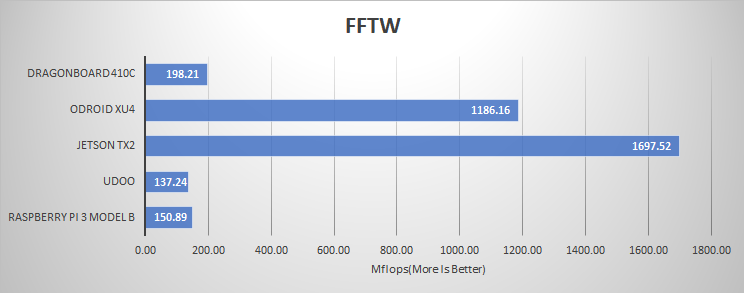
\includegraphics[scale=1]{./resultphoronix/fftw.png}
\end{figure} 

\begin{figure}[H]
\center
\caption{FFTW/Cost benchmark.\label{fig:FFTW_cost}}
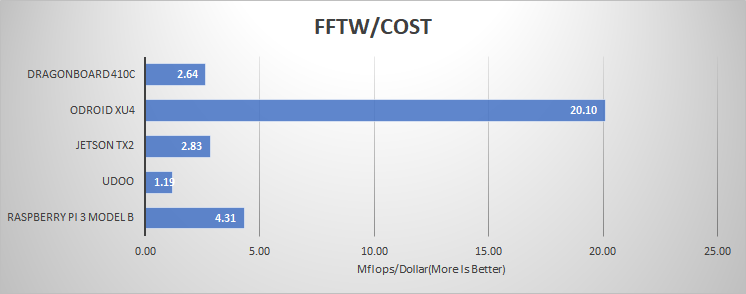
\includegraphics[scale=1]{./resultphoronix/fftw_cost.png}
\end{figure} 

\subsubsection{John The Ripper}
John The Ripper algorithm is a password cracker. The odroid Xu4 scored the best in the benchmark as well as the cost benchmark . 
The worst one is the Udoo board(\ref{fig:john}). The worst value for money board is the Jetson TX2 (\ref{fig:john_cost}).

\begin{figure}[H]
\center
\caption{John The Ripper benchmark.\label{fig:john}}
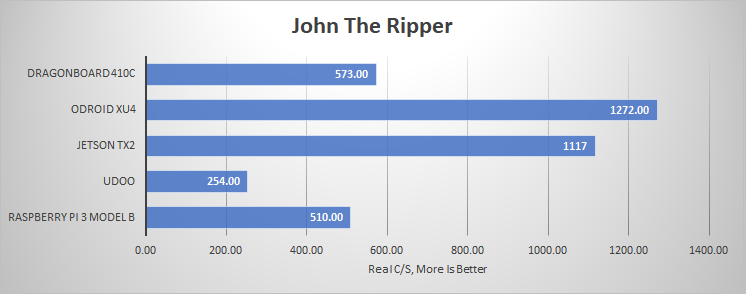
\includegraphics[scale=1]{./resultphoronix/john.png}
\end{figure} 

\begin{figure}[H]
\center
\caption{John The Ripper / Cost benchmark.\label{fig:john_cost}}
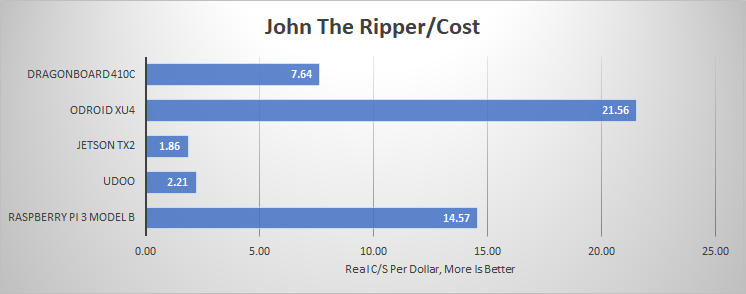
\includegraphics[scale=1]{./resultphoronix/john_cost.png}
\end{figure}

\subsubsection{C-ray}
The C-Ray is a raytracer it is used to test the floating-point CPU performance. The one used on this benchmark is multi-threaded(16 threads per core). It will generate a 1600 x 1200 image and will shoot 8 rays per pixel for anti-aliasing. \cite{OpenBenc27:onlineCRAY}

The Jetson TX2 scored the best on the benchmark but the Odroid Xu4 Has the best price value score.

\begin{figure}[H]
\center
\caption{C-Ray benchmark.\label{fig:cray}}
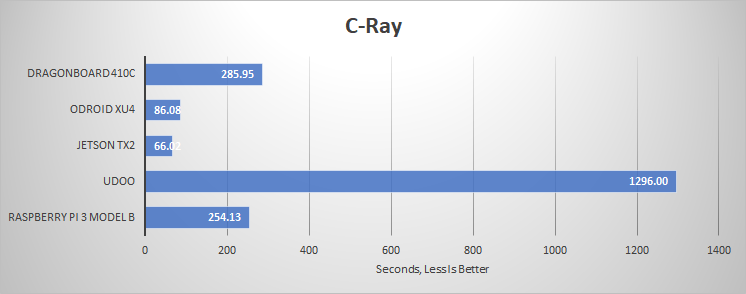
\includegraphics[scale=1]{./resultphoronix/cray.png}
\end{figure} 

\begin{figure}[H]
\center
\caption{C-Ray/Cost benchmark.\label{fig:cray_cost}}
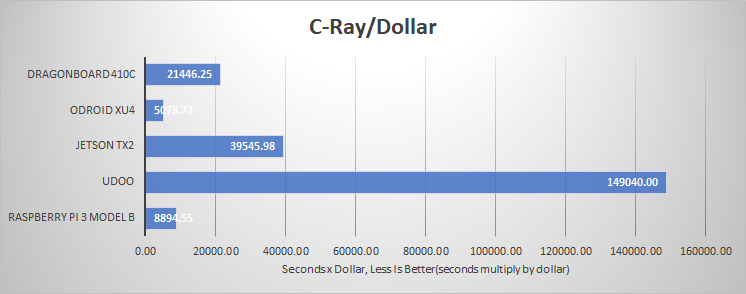
\includegraphics[scale=1]{./resultphoronix/cray_cost.png}
\end{figure} 

\subsubsection{Smallpt}
%Smallpt is a C++ global illumination renderer written in less than 100 lines of code. Global illumination is done via unbiased Monte Carlo path tracing and there is multi-threading support via the OpenMP library. \cite{OpenBenc95:onlinesmall}

The Odroid Xu4 scored the best it has the best result in for the value benchmark but the jetson has the best performance. 


\begin{figure}[H]
\center
\caption{smallpt benchmark.\label{fig:smallpt}}
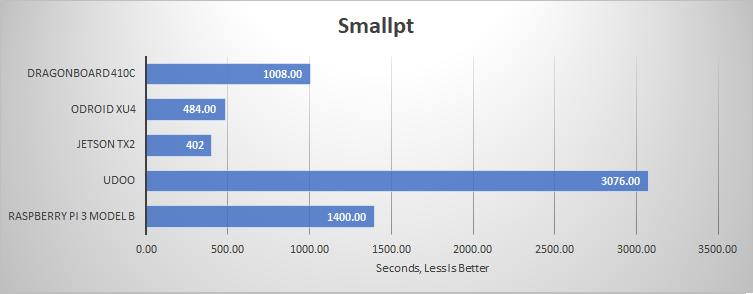
\includegraphics[scale=1]{./resultphoronix/smallpt.png}
\end{figure} 

\begin{figure}[H]
\center
\caption{smallpt/cost benchmark.\label{fig:smallpt_cost}}
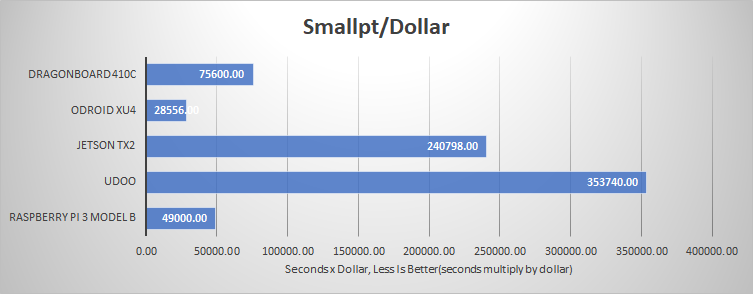
\includegraphics[scale=1]{./resultphoronix/smallpt_cost.png}
\end{figure}

\subsubsection{FLAC Audio Encoding}

\begin{figure}[H]
\center
\caption{flac audio benchmark.\label{fig:flacAduio}}
\includegraphics[scale=1]{./resultphoronix/flacAudio.png}
\end{figure}

\begin{figure}[H]
\center
\caption{flac audio /cost benchmark.\label{fig:FlacAudioCost}}
\includegraphics[scale=1]{./resultphoronix/flacAudio_cost.png}
\end{figure}


\subsubsection{Redis}

\begin{figure}[H]
\center
\caption{Redis(Set) benchmark.\label{fig:redisSet}}
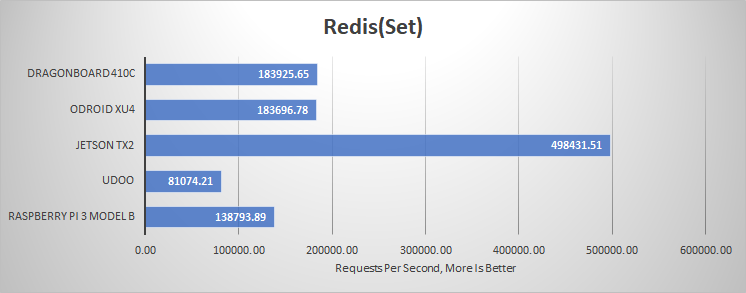
\includegraphics[scale=1]{./resultphoronix/redisSet.png}
\end{figure}

\begin{figure}[H]
\center
\caption{Redis(set)/cost benchmark.\label{fig:redisSet_cost}}
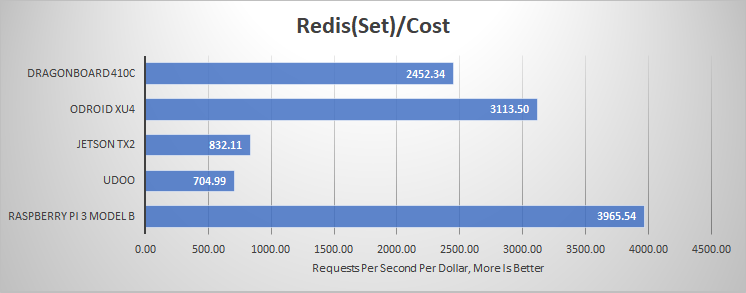
\includegraphics[scale=1]{./resultphoronix/redisSet_cost.png}
\end{figure}

\begin{figure}[H]
\center
\caption{Redis(Get) benchmark.\label{fig:redisGet}}
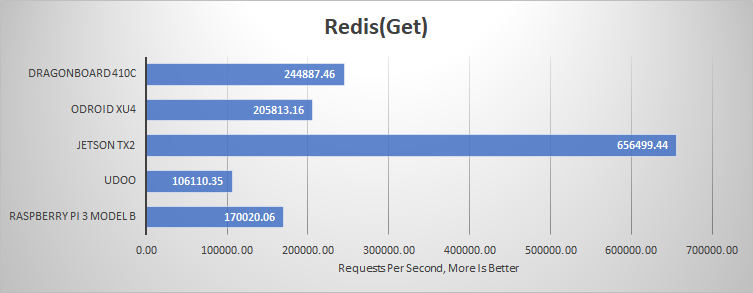
\includegraphics[scale=1]{./resultphoronix/redisGet.png}
\end{figure}

\begin{figure}[H]
\center
\caption{Redis(Get)/cost benchmark.\label{fig:redisGet_cost}}
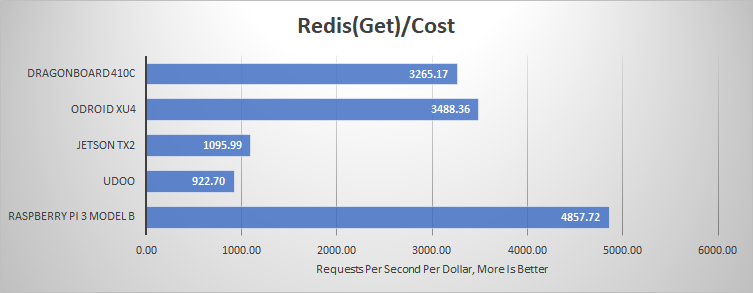
\includegraphics[scale=1]{./resultphoronix/redisGet_cost.png}
\end{figure}

\subsubsection{Himeno}

\begin{figure}[H]
\center
\caption{Himeno benchmark.\label{fig:himeno}}
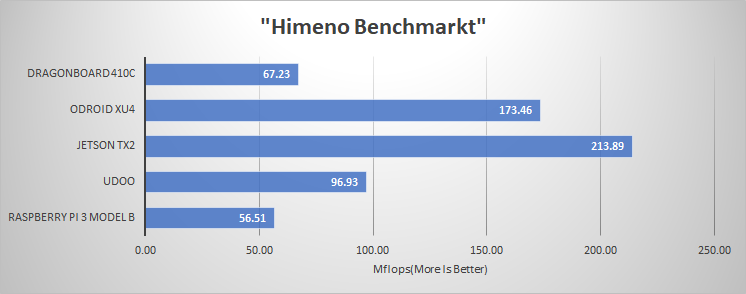
\includegraphics[scale=1]{./resultphoronix/himeno.png}
\end{figure}

\begin{figure}[H]
\center
\caption{Himeno/cost benchmark.\label{fig:himeno_cost}}
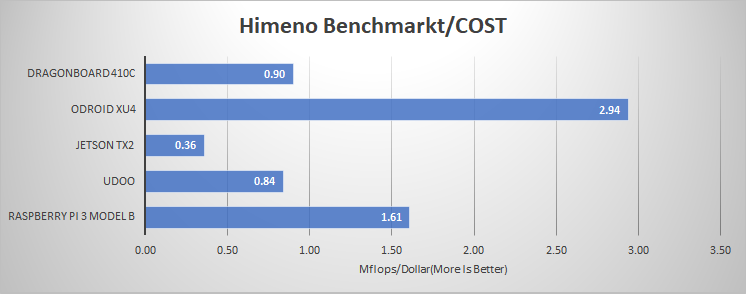
\includegraphics[scale=1]{./resultphoronix/himeno_cost.png}
\end{figure}

\subsubsection{conlusion}

In all the processors benchmarks the best board is without surprise the Jetson TX2. The reason is because this board is more powerful it has 8Gb of rams compared to the Odroid Xu4 it has 4 times the amount of ram memory. 
The best price value board is the Odroid Xu4 for performance. Its scores much better than all the other board for the Performance benchmarks.

For the Redis benchmarks wich is a system benchmark. The Jetson still score the best but on the Rasperry Pi3 score the best in term of price value. 
All the result are available on following link : \url{https://openbenchmarking.org/result/1805273-FO-1805279FO65}\\


%\begin{figure}[H]
%\center
%\caption{meta benchmark.\label{fig:meta}}
%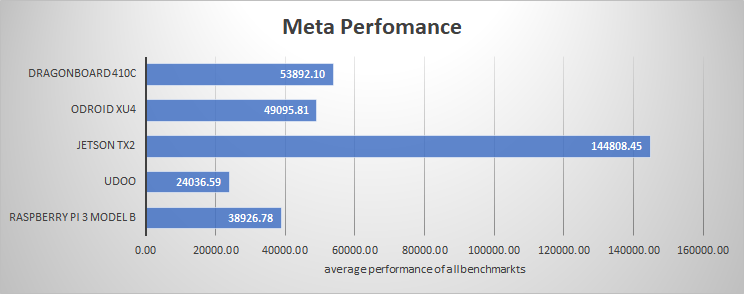
\includegraphics[scale=1]{./resultphoronix/meta.png}
%\end{figure}
%
%\begin{figure}[H]
%\center
%\caption{meta/cost benchmark.\label{fig:himeno_cost}}
%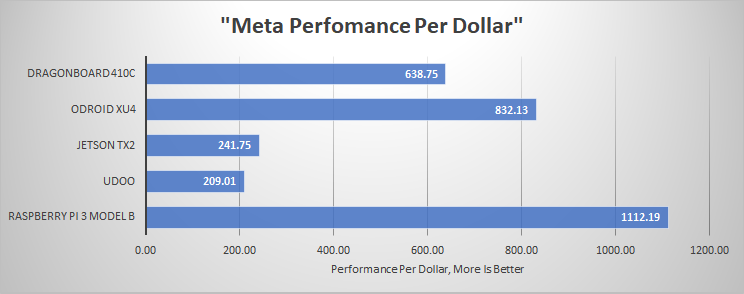
\includegraphics[scale=1]{./resultphoronix/meta_cost.png}
%\end{figure}


%lite conclusion on existing benchmarkts 
The user has do decides if he want to save money and work with a board like a  Raspberry Pi 3 or get maximum performance and work with a jetson board.A good compromise is the Odroid Xu4. This board looks powerful and is low cost. \\

%conclusion of existing benchmarks

About vision we can find a lot of benchmarks that compares algorithms to do some specific task like face-detection. There are also more general benchmarks that compares single boards computers (\ref{SBC}), but there is no benchmark that will compare boards on how they are good to do real time image processing.

\chapter{Pixy cam}

The pixycacam is an vision sensor. This board can help an arduino or simal board to do fast image processing. the pixicam will process the image and send only useful information to the microcontroller. The frame rate is 50Hz and it can use several interfaces to send the inforamtion:UART serial, SPI, I2C, USB, or digital/analog output. In our use cas the pixi will do the iamge processing while the micronctorller(Arduino) can use his CPU for other tasks.\cite{pixy}

\begin{description}
	\item[Technical specs:]
\end{description}
\begin{itemize}
\item Processor: NXP LPC4330, 204 MHz, dual core
\item Image sensor: Omnivision OV9715, 1/4", 1280x800
\item Lens field-of-view: 75 degrees horizontal, 47 degrees vertical
\item Lens type: standard M12 (several different types available)
\item Power consumption: 140 mA typical
\item Power input: USB input (5V) or unregulated input (6V to 10V)
\item RAM: 264K bytes
\item Flash: 1M bytes
\item Available data outputs: UART serial, SPI, I2C, USB, digital, analog
\item Dimensions: 2.1" x 2.0" x 1.4
\item Weight: 27 grams
\end{itemize}

\section{Limit of Pixy}

The Pixy can only be used for color detection not for object detection. The second problem is that the Pixy can only detect flashy colors like red yellow blue (figure: \ref{fig:redcolor}). If the object has any rebound color the Pixy will not detect the object (figure:\ref{fig:reboundColor}). Last point is that the pixy will not detect white colors (figure: \ref{fig:whitecolor}). 

\begin{figure}[H]
\center
\caption{Red color detection.\label{fig:redcolor}}
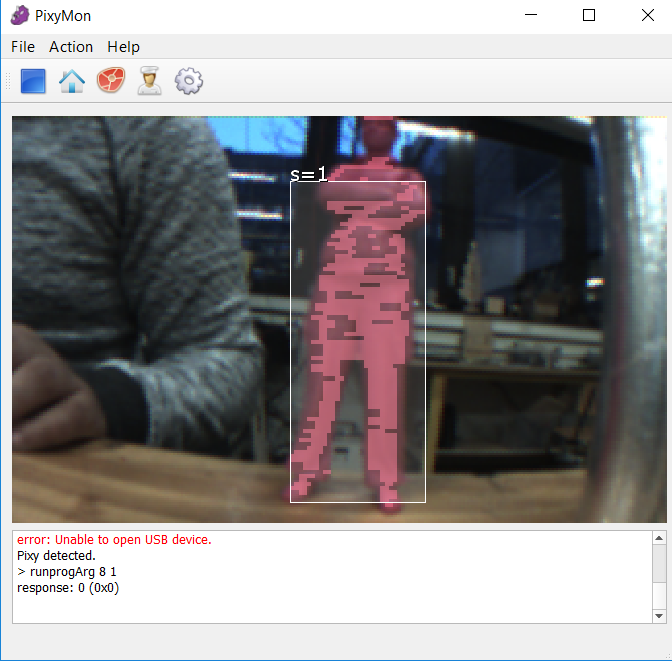
\includegraphics[scale=0.5]{./img/pixyRedcolor}
\end{figure} 


\begin{figure}[H]
\center
\caption{Rebound object detection.\label{fig:reboundColor}}
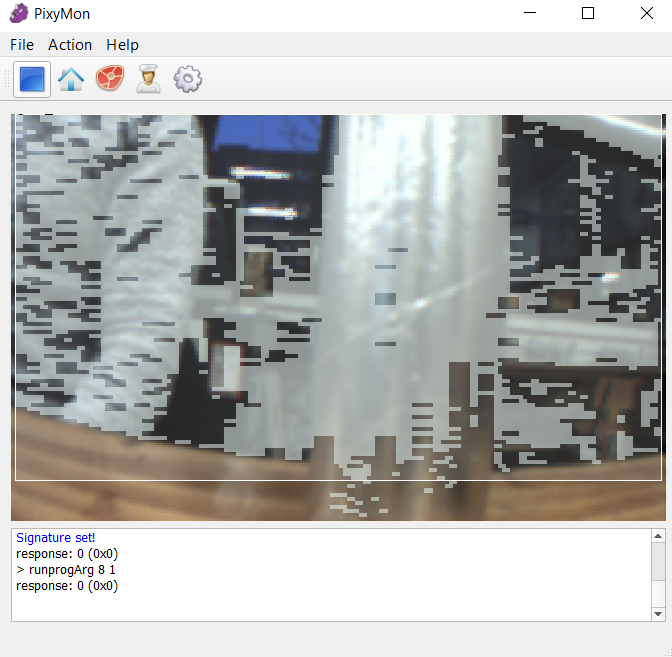
\includegraphics[scale=0.5]{./img/pixyAluminuim}
\end{figure} 

\begin{figure}[H]
\center
\caption{white color detection.\label{fig:whitecolor}}
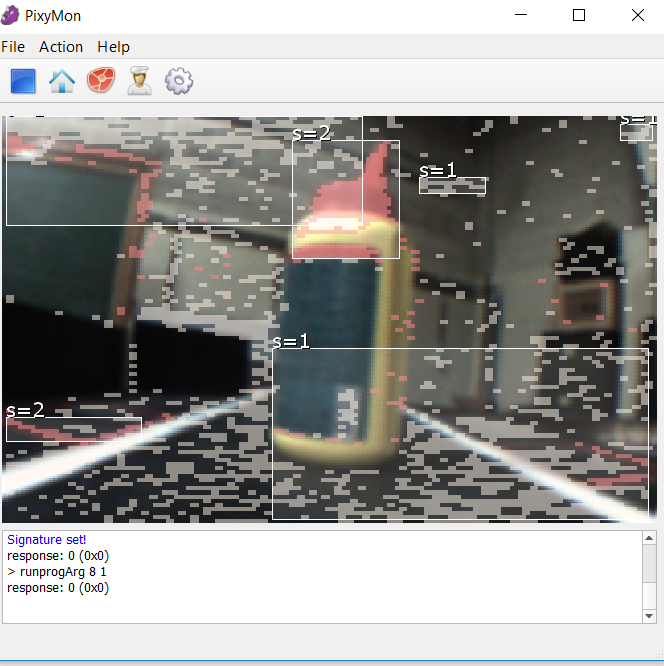
\includegraphics[scale=0.5]{./img/whitecolor}
\end{figure} 







\chapter{Comparison}
\section{board comparison}

This thesis will compare 5 boards. The chosen boards all run an arm architecture. The boaérd are selected because of they popularity, price(depending on use case) and power consumption:
\begin{itemize}
\item \textbf{Raspberry Pi 3}: The most famous single board computer of our list. The cost of the board is around \$35. It is possible to run several operating system on it like Linux or Windows 10 IOT core. \cite{Raspberr76:online}

\item \textbf{Udoo}: The Udoo Dual is a computer that can be used with Android and Linux. It is a powerful prototyping board because it contains a processor and a Arduino Due microcontroller. To summerize the Udoo we can say that it bring the best of an Raspberry Pi and an Arduino togheter in-to one single board.  \cite{maksimovic2014raspberry}
On the market we can find three type of Udoo that combine a processor and an Arduino. In this thesis we will discuss the Udoo dual. The dual is the mid-range Udoo and the cost of it is around \$115 \cite{DUALQUAD20:online}.

\item \textbf{Odroid Xu4}: The Odroid X4 is and powerful Single board computer. It combine two processor a Samsung Exynos5422 Cortex A15 (2 GHz) and a Cortex A7 Octa core CPU (1.4 Ghz). This two processors are combined with 2 GB of RAM. \cite{abdullah2016position} The board can run several flavors of Linux. The computing power of the X4 seems to be seven times faster than the Raspberry Pi3. 
The Xu4 can be found on the market at the price of \$59. \cite{ODROIDHa46:online}

\item \textbf{Dragonboard 410c}: The Dragonboard 410 c is a single board computer basd on the  mid-tier Qualcomm® Snapdragon™ 410E processor. It can run Windows 10 IOT core and Linux(Andoid, Debian). The price is around \$75. \cite{DRAGONBO86:online}  

\item \textbf{Nvidia jetston tx2}: Jetson is an NVIDIA® high performane computer. it is low-power and it is ideal for embedded compute-intensive projects like deep learning or computer vision. \cite{JetsonFA42:online}  This thesis will compare the Jetson TX2 Developer Kit  with other boards. On the market the TX2 Devloper kit can bi found for \$599.

Table \ref{comparaison board table} compares the technical specs of all the cited boards.
\newpage
  \null

\end{itemize}
% Please add the following required packages to your document preamble:
% \usepackage{graphicx}
\begin{table}[]
\centering
\resizebox{1\textwidth}{!}{%
\begin{tabular}{p{3.5cm}|p{3cm}p{3cm}p{3cm}p{3cm}p{3cm}p{3cm}}
 & \textbf{udoo dual}   & \textbf{ raspberry pi 3} & \textbf{odroid Xu} &\textbf{ Dragonboard 410c} & \textbf{NVIDIA\newline jetston TX2 \newline devlopper kit} & \textbf{Pixycam}   \\
 \hline
\textbf{cpu} & NXP i.MX 6 DualLite \newline Atmel SAM3X8E (Arduino Due) & ARM Cortex-A53 Quad-core & Samsung Exynos5422 Cortex™A15 2Ghz \newline + Cortex™-A7 Octa core CPUs & ARM Cortex-A53 Quad-core & HMP Dual Denver 2/2MB L2 + Quad ARM A57/2MB L2 & NXP LPC4330 \\

\# cores & 2 & 4 & 8 & 4 & 6 & 2 \\

clk(GHz) & 1 & 1.2 & 2 & 1.2 & 2 & 0.204 \\
ram(GB) & 1 & 1 & 2 & 1 & 8 & 0.000264 \\
memory(GB) & unlimitted ( sd card) & unlimitted ( sd card) & unlimitted ( sd card) & unlimitted ( sd card) & 32 & 1M \\
ipc(instruction per cycles) & 1 & 1 & 1 & 1 & 1 & 1 \\
GFLOPs & 2 & 4.8 & 16 & 4.8 & 12 & 0.408 \\
Power supply\newline(DC V) & 6 & 5 & 5 & 6.5 & 19 &  \\
 &  &  &  &  &  &  \\
\textbf{GPU} & yes & yes & yes & yes & yes & no \\
 & Vivante GC 880 + Vivante GC 320 & broadcom videocore 4 & mali T628 & Qualcomm Ardeno 306 & NVIDIA Pascal, 256 NVIDIA CUDA Cores &  \\
opencl/cuda & maybe & no & yes & yes & yes(Cuda) &  \\
core clk (mhz) & 400 & 250 & 600 & 450 &  &  \\
pixel/rate(Mpixel/ sec) & 80 & 1000 &  &  &  &  \\
 &  &  &  &  &  &  \\
operating System & Linux & linux \newline windows10 & linux & linux \newline windows & linux & no \\
 & debian & debian & debian & debian & debian &  \\
camera plug & yes & yes & yes & yes & yes &  \\
 &  &  &  &  &  &  \\
python /opencv & yes & yes & yes & yes & yes &  \\
 &  &  &  &  &  &  \\
price(€) & 110 & 40 & 75 & 75 & 599 &  \\
 &  &  &  &  &  &  \\
arduino compatible\newline(connector for Arduino) & yes & no & no & yes & no & yes
\end{tabular}%
}
\caption{Comparison board table \cite{SamsungE46:online} \cite{VideoCor59:online} \cite{iMX6Solo72:online} \cite{JetsonFA42:online} } 
\label{comparaison board table}
\end{table}
%\section{Camera comparison}


\chapter{Generic vision Benchmark}
facedetection, colordetection, openCl, edgedetection, convolution, matrixmultiplucation

\chapter{Results}   


\chapter{Conclusion}

 
\setstretch{1.0}
\printbibliography
\thispagestyle{plain}
\newpage
\phantomsection
\chapter{Appendix}
\appendix


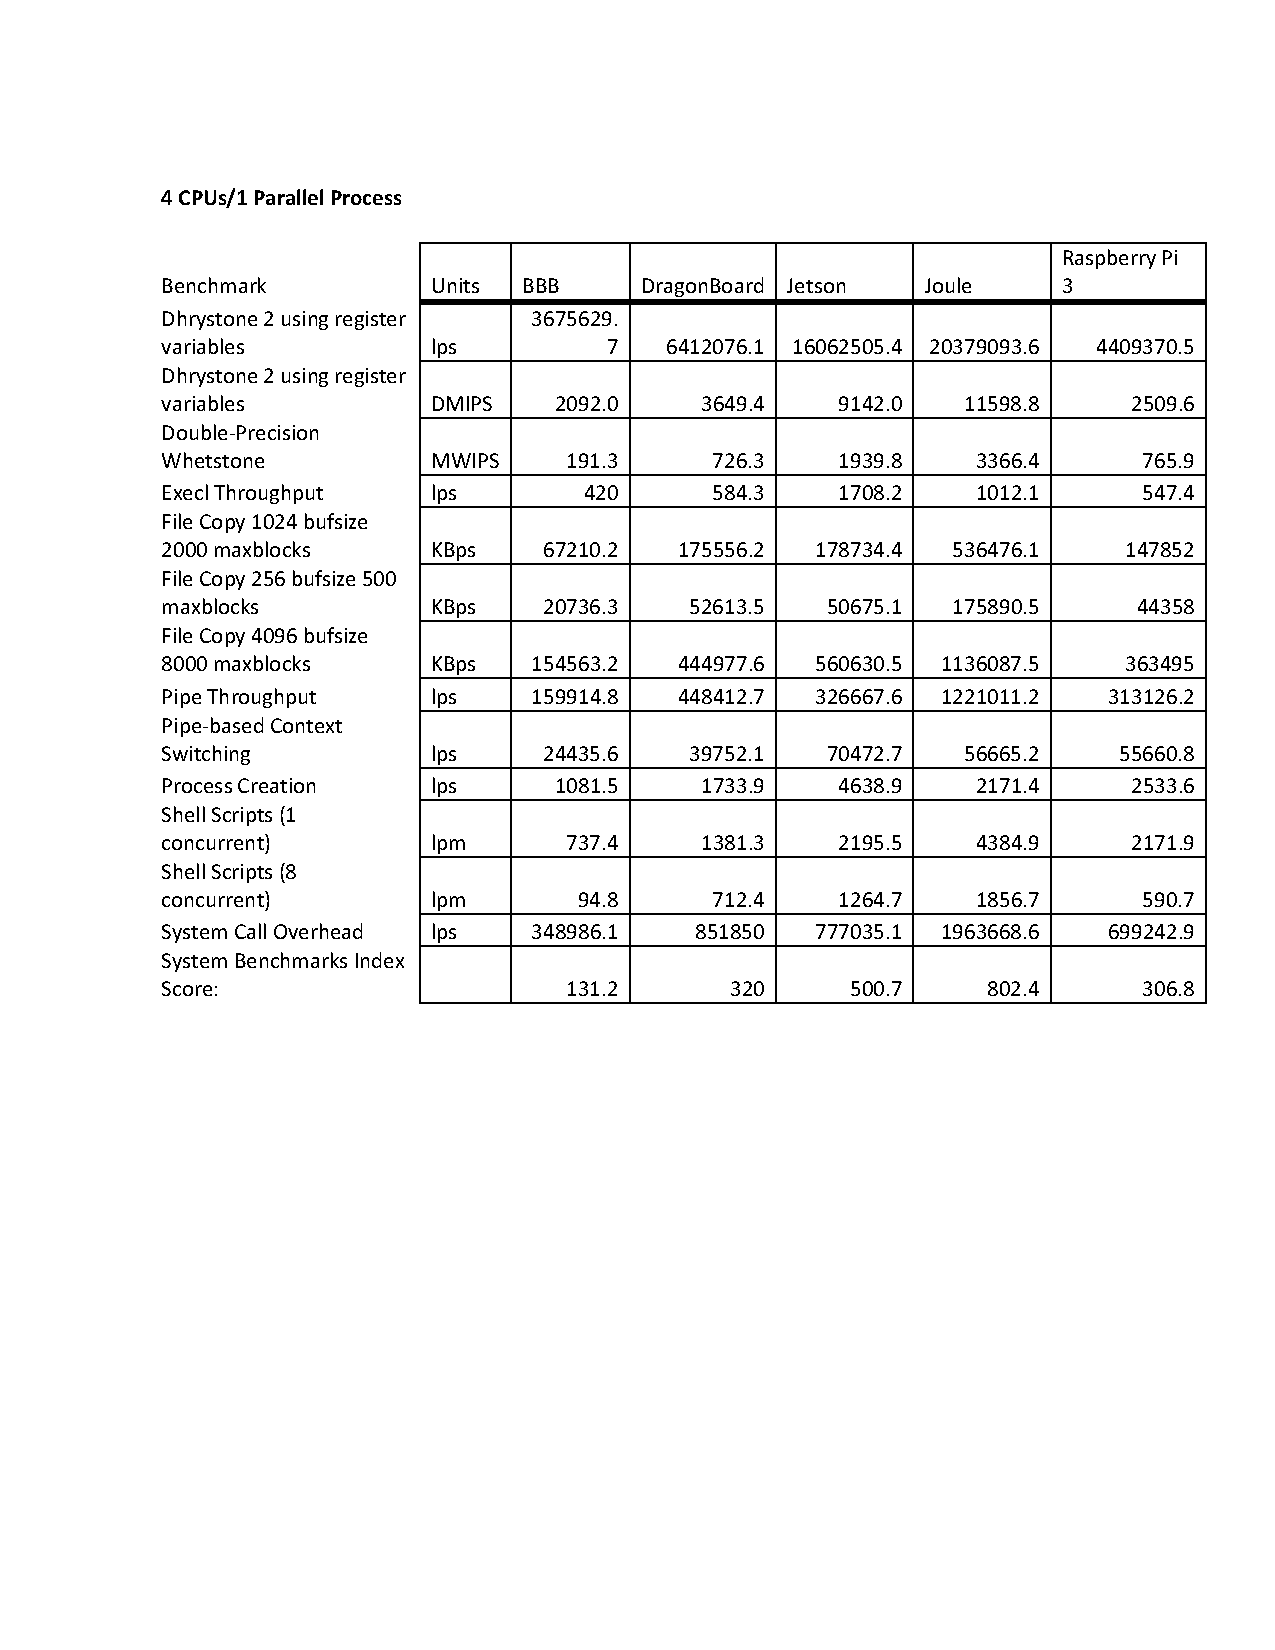
\includepdf[scale=0.8,pages=-,pagecommand=\section{Appendix 1 : Result benchmark \cite{Benchmar1:online} \label{chap:appendix1}}]{./appendix/SBCArrow.pdf}


\end{document}
